%----------------------------------------------------------------------------------------
%	METODE
%----------------------------------------------------------------------------------------
\section*{METODE PENELITIAN}
\subsection*{Data Penelitian}
Data yang digunakan dalam penelitian ini adalah data titik panas di Provinsi Riau dari tahun 2001 sampai 2015 yang diperoleh dari \textit{Fire Information for Resource Management System} (FIRMS) MODIS NASA. Aspek yang diamati pada data titik panas adalah aspek spasial kemunculan titik panas bulanan. Field  yang digunakan adalah field lattidude, longitude, brightness, scan, track, acqdate, acqtime, satellite, confidence, version, brightt31, dan frp  seperti yang ditunjukan pada tabel \ref*{titikpanas}.

% Please add the following required packages to your document preamble:
% \usepackage{booktabs}
\begin{table}[h]
	\centering
	\caption{\textit{Field} data titik panas}
	\label{titikpanas}
	\begin{tabular}{@{}ll@{}}
		\toprule
		Field       & Value    \\ \midrule
		LATITUDE    & -0.747   \\
		LONGITUDE   & 100.915  \\
		BRIGHTNESS  & 312.2    \\
		SCAN        & 2.4      \\
		TRACK       & 1.5      \\
		ACQ\_DATE   & 1/1/2012 \\
		ACQ\_TIME   & 624      \\
		SATELLITE   & A        \\
		CONFIDENCE  & 49       \\
		VERSION     & 5.1      \\
		BRIGHT\_T31 & 295      \\
		FRP         & 29.6     \\ \bottomrule
	\end{tabular}
\end{table}

Penjelasan \textit{field}  Tabel \ref{titikpanas} yaitu:
Lattidude adalah Koordinat lintang
Longitude adalah Koordinat bujur 
Brightness adalah Suhu kecerahan, diukur dalam Kelvin menggunakan saluran MODIS 
21/22 dan saluran 31.
Scan Track adalah Resolusi spasial yang sebenarnya dari pixel dipindai. Meskipun algoritma 
bekerja pada 1 km resolusi, piksel MODIS mendapatkan lebih besar ke tepi 
scan.
AcqDate	adalah Tanggal akuisisi pixel titik panas aktif.
AcqTime	adalah Waktu layang satelit di UTC.
Satellite adalah Jenis satelit yang mendeteksi. Satelit Terra atau Aqua.
Confidence adalah Tingkat kepercayaan dari tiap pixel api yang aktif.
Version	adalah Versi yang mengidentifikasikan koleksi data.
BrightT31 adalah Saluran 31 suhu kecerahan (dalam Kelvin) dari pixel titik panas yang aktif.
Frp adalah Fire Radiative Power, Menggambarkan kekuatan radiasi api pixel-
terintegrasi dalam MW (megawat). FRP memberikan informasi mengenai output panas radiasi diukur dari kebakaran terdeteksi. Jumlah energi panas radiasi dibebaskan per satuan waktu (Fire Radiative Power) diduga terkait dengan tingkat dimana bahan bakar yang dikonsumsi


\subsection*{Tahapan Penelitian}
Tahapan-tahapan yang dilakukan pada penelitian ini dapat dilihat pada Gambar 1.

\begin{figure}[h!] % Gunakan \begin{figure*} untuk memasukkan Gambar
\centering
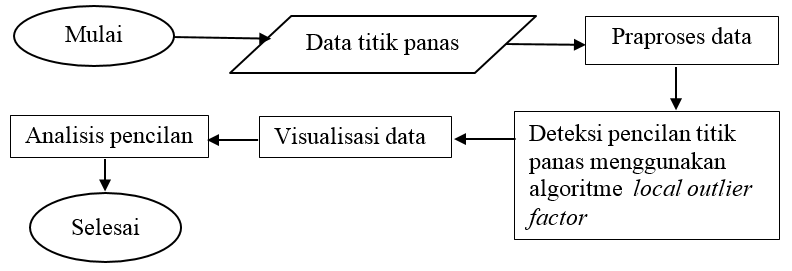
\includegraphics[width=230pt]{tahapanPenelitian.png}
\caption{Tahapan penelitian}
\label{fig:tahapan}
\end{figure}

\subsubsection*{a. Pengumpulan Data}
Data yang digunakan dalam penelitian ini adalah data titik panas di Provinsi Riau dari tahun 2001 sampai 2015 yang diperoleh dari FIRMS MODIS NASA. Data titik panas terdiri dari data titik panas tahun 2001 hingga tahun 2015 di wilayah Provinsi Riau. Data tersebut terdiri dari atribut latitude, longitude, brightness, scan, track, acqdate, acqtime, satellite, confidence, version, brightt31, frp. Setiap barisnya menjelaskan satu kemunculan titik panas yang diperoleh dari pengindraan jarak jauh menggunakan sensor MODIS. 
	 
\subsubsection*{b. Praproses Data}
Menurut Han et al (\citeyear{Han2012}) “dalam tahap praproses data, terdapat beberapa tahap utama, yaitu pembersihan data, pengintegrasian data, seleksi data, dan transformasi data”. Dalam penelitian ini dilakukan pembersihan dan transformasi data. Pembersihan data dilakukan untuk memilih data titik panas yang berada di Provinsi Riau juga memilih peta Provinsi Riau dari peta kabupaten dan kota se-Indonesia. Langkah ini dilakukan untuk menghilangkan data titik panas yang berada di luar Provinsi Riau. Tahap ini dilakukan menggunakan perangkat lunak PostgreSQL, PostGIS 2.0 \textit{Shapefile} and DBF \textit{Loader Eksporter}, dan Quantum GIS.
Setelah data bersih, kemudian data titik panas pada tahun 2001 hingga 2015 dipilih  menggunakan queri pada DBMS PostgreSQL dan dilakukan transformasi data yaitu agregasi data. Agregasi data adalah operasi penjumlahan jumlah kejadian titik panas menjadi data harian, bulanan ataupun tahunan. 

\subsubsection*{c. Deteksi Pencilan Titik panas Menggunakan Algoritme \textit{Local Outlier Factor}}
Dalam tahapan ini diterapkan fungsi \textit{local outlier factor} pada perangkat lunak R. Fungsi tersebut diberikan masukkan atau argumen berupa data frekuensi titik panas harian dari tahun 2001 hingga 2015 juga nilai k sebesar 2 hingga 10. 
Local outlier factor  adalah algoritme deteksi outlier berdasarkan jarak tetangga lokal  (\cite{Beunig2010}). \textit{Local outlier factor} tidak menggunakan distribusi data \textit{global} . Pada Gambar 2 dapat dilihat O1 dan O2 adalah \textit{local outlier} C1, O3 adalah \textit{global outlier}. Dengan pendekatan \textit{clustering} O1 dan O2 tidak dapat terdeteksi sebagai \textit{outlier}.



\begin{figure}[h!] % Gunakan \begin{figure*} untuk memasukkan Gambar
	\centering
	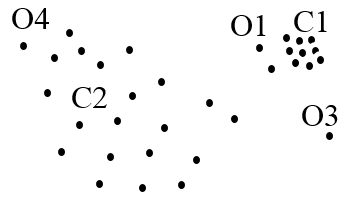
\includegraphics[width=190pt]{sebaranTitik.png}
	\caption{Sebaran data}
	\label{fig:sebaranTitik}
\end{figure}

 Ilustrasi \textit{local outlier}  dapat dilihat pada Gambar 2.\textit{ Local outlier factor } menghitung jarak maksimum dari jarak tetangga dengan jumlah tetangga yang didefinisikan oleh pengguna.Notasinya sebagai berikut (\cite{Beunig2010}):


\begin{equation}
	reach-dist\space k(p, o) = \max \{\space  k-\textit{distance}(o), d(p, o) \}.
\end{equation}
dengan
k 	adalah jumlah tetangga dan \textit{distance} adalah fungsi jarak. Sebuah objek local outlier factor  adalah rasio rataan dari o degan jarak k-ketetanggan lokal terdekat.Notasinya sebagai berikut (\cite{Beunig2010}):

\begin{equation}
lrd_{MinPts}(p) = 1/(\frac{\displaystyle\sum_{o \epsilon N_{MinPts}(p)}  reach-dist_{MinPts}(p,o) } { N_{MinPts}(p)} )
\end{equation}

\begin{equation}
LOF_{MinPts}(p)= \frac{\displaystyle\sum_{o \epsilon N_{MinPts}(p)} \frac{lrd_{MinPts}(o)}{lrd_{MinPts}(p)}}{N_{MinPts}(p)}
\end{equation}

dengan lrd adalah \textit{local reachability density} dan LOF adalah \textit{local outlier factor}.

\subsubsection*{d. Visualisasi Data}
Pada tahapan ini data yang diolah dengan algoritme \textit{local outlier factor} divisualisasikan pada peta sehingga dapat terlihat dengan mudah data mana saja yang termasuk pencilan.

\subsubsection*{e. Analisis Pencilan}
Pada tahap ini diperlihatkan objek-objek pencilan dari data penelitian. Data hasil deteksi pencilan dianalisis untuk mengetahui informasi yang terdapat pada data seperti ukuran pemusatan dan tanggal-tanggal yang terdeteksi pencilan.

\subsection*{Lingkungan Pengembangan}
Spesifikasi perangkat keras dan perangkat lunak yang digunakan dalam penelitian ini adalah sebagai berikut :
\begin{enumerate}[noitemsep] 
	\item Perangkat keras berupa komputer personal dengan spesifikasi 
	\begin{itemize}
			\item Prosesor Intel(R) Core(TM) i7-5500U  2.40GHz
			\item RAM 12288 MB.
	\end{itemize}
		\item Perangkat lunak
		\begin{itemize}
			\item Komputasi statistika R versi 3.2.0.
			\item RStudio versi 0.98.1103.
			\item PostgreSQL dengan ekstensi PostGIS.
			\item Pengolah data spatial Quantum GIS 2.6.1.
			\item Microsoft Excel.
			\item PostGIS 2.0 \textit{Shapefile} and DBF \textit{Loader Eksporter}.
			\item Library DMwR pada perangkat lunak R.
		\end{itemize}
\end{enumerate}





\subsection*{Jadwal Kegiatan}
Jadwal pernelitian dimulai dari bulan April 2015 sampai dengan Desember 2015. Ilustrasi penjadwalan dapat dillihat pada Tabel \ref{Rencana}.
% Please add the following required packages to your document preamble:
% \usepackage{booktabs}
% \usepackage{multirow}
% \usepackage[table,xcdraw]{xcolor}
% 
% If you use beamer only pass "xcolor=table" option, i.e. \documentclass[xcolor=table]{beamer}

\begin{table*}[h!]
	\begin{center}
	\caption{Rencana jadwal penelitian}
	\label{Rencana}
	\begin{tabular}{@{}llllllllll@{}}
		\toprule
\multicolumn{1}{c}{}                               & \multicolumn{9}{c}{{\bf Tahun 2015}}                                                                                                                                                                                                             \\ \cmidrule(l){2-10} 
\multicolumn{1}{c}{\multirow{-2}{*}{{\bf Jadwal}}} & April                    & Mei                      & Juni                     & Juli                     & Agus                     & Sept                     & Okt                      & Nov                      & Des                      \\ \cmidrule(r){1-10}
		Pengumpulan data                                     & \cellcolor[HTML]{000000}   & \cellcolor[HTML]{000000} &                           &                           &                           &                           &                          &                          &                          \\
		Praproses data                                       &                            &                          & \cellcolor[HTML]{000000}  & \cellcolor[HTML]{000000}  &                           &                           &                          &                          &                          \\
		Kolokium                                             &                            &                          & \cellcolor[HTML]{000000}  &                           &                           &                           &                          &                          &                          \\
		Implementasi \textit{Local outlier factor}           &                            &                          &                           & \cellcolor[HTML]{000000}  & \cellcolor[HTML]{000000}  & \cellcolor[HTML]{000000}  & \cellcolor[HTML]{000000} & \cellcolor[HTML]{000000} &                          \\
		Evaluasi hasil penelitian                            &                            &                          &                           &                           &                           &                           &                          & \cellcolor[HTML]{000000} &                          \\
		Penyusunan skripsi dan makalah seminar               &                            &                          &                           &                           &                           &                           & \cellcolor[HTML]{000000} & \cellcolor[HTML]{000000} & \cellcolor[HTML]{000000} \\
		Seminar                                              &                            &                          &                           &                           &                           &                           &                          & \cellcolor[HTML]{000000} & \cellcolor[HTML]{000000} \\
		Sidang tugas akhir                                   &                            &                          &                           &                           &                           &                           &                          &                          & \cellcolor[HTML]{000000} \\
		Revisi Skripsi dan penyelesaian                      &                            &                          &                           &                           &                           &                           &                          &                          & \cellcolor[HTML]{000000} \\
		Surat Keterangan Lulus (SKL)                         &                            &                          &                           &                           &                           &                           &                          &                          & \cellcolor[HTML]{000000} \\
		\bottomrule
	\end{tabular}
		\end{center}
\end{table*}




